\chapter{The Tower of Hanoi with ROS}
\section{Important}
Read the entire lab before starting and especially the ``Grading" section so you are aware of all due dates and requirements associated with the lab.  Hopefully you are reading this well before your lab section meets as given the compressed schedule, it is very important that you arrive at lab well prepared.  This semester, the more you do prior to your lab session, the more you will get out of the short time you have with the TA.
% \todo[inline]{Need to change these}
\section{Objectives}
This lab is an introduction to controlling the UR3e robot using the Robot Operating System (ROS) and the Python programming language.  In this lab, you will:
\begin{itemize}
% \item Record joint angles that position the robot arm at waypoints in the Tower of Hanoi solution
\item Modify the given starter python file to move the robot to waypoints and enable and disable the suction cup gripper such that the blocks are moved in the\
correct pattern.
\item If the robot suction senses that a block is not in the gripper when it should be, the program should halt with an error.
\item Program the robot to solve the Tower of Hanoi problem allowing the user to select any of three starting positions and ending positions.
\end{itemize}

\newpage
\section{Pre-Lab}
Read ``\textit{A Gentle Introduction to ROS}", available online, Specifically:
\begin{itemize}
\item Chapter 2: 2.4 Packages, 2.5 The Master, 2.6 Nodes, 2.7.2 Messages and message types.
\item Chapter 3 Writing ROS programs.
\end{itemize}
\section{References}
\begin{itemize}
\item Consult Appendix \ref{cprog} of this lab manual for details of ROS and Python functions used to control the UR3e.
\item ``\textit{A Gentle Introduction to ROS}", Chapter 2 and 3. \url{http://coecsl.ece.illinois.edu/ece470/agitr-letter.pdf}
% I can't find this anymore Fall 2020
% \item A short tutorial for ROS by Hyongju Park. \url{https://sites.google.com/site/ashortrostutorial/}
\item \url{http://wiki.ros.org/}
\item Since this is a robotics lab and not a course in computer science or discrete math, feel free to Google for solutions to\
the Tower of Hanoi problem.\footnote{\url{http://www.cut-the-knot.org/recurrence/hanoi.shtml} (an active site, as of this writing.)} You\
are not required to implement a recursive solution.

\end{itemize}

\newpage
\section{Task}
% \todo[inline]{I think we should describe traditional TOH and then explain how ours works.  We also will want figures.}
\subsection{Standard Tower Of Hanoi}
As you hopefully know by now, the normal way that the Tower of Hanoi puzzle is set up is as a stack of discs or blocks as seen in \figref{towers}.  This makes many of the rules obvious such as that you cannot move a lower block while a higher block still rests on it.  This arrangement is hard to simulate in Gazebo (The simulator we will be using).  Stacked blocks do not behave in a stable manner and thus it is difficult to create neat stacks without disturbing/toppling them.  As an alternative, we have modified the puzzle to work with the simulator.

\subsection{Simulated Tower Of Hanoi}
In our version of Tower of Hanoi, we have laid the blocks flat on the table as seen in \figref{towers2d}.  Now, instead of rising vertically from the table, the blocks ``rise" as they move farther from the viewer.  Thus the ``towers" form the columns of a grid, while the ``height" depends on the rows of the grid.  We will make use of this matrix like structure to organize our waypoints in the code.
% The original goal of Tower of Hanoi is to move a ``tower'' of three blocks from one of three locations on the table to another. Due to the limitations of simulator, the tower is "2D" (lying on the table) instead of 3D one which you stack vertically. So instead of stacking the blocks upwards, you are "stacking" the blocks towards the robot base horizontally. 

% An example is shown in \figref{towers}.  The blocks are numbered with block 1 on the top and block 3 on the bottom. The blocks are color-coded in the simulator, and it corresponds to the numbers in the following order:

Color has been used to help keep track of the blocks in the simulator:
\begin{enumerate}
    \item Red - Top Block
    \item Yellow - Middle Block
    \item Green - Bottom Block
\end{enumerate}

This "2D" version doesn't have gravity to enforce building from "bottom" to "top", but you should still code it as if it has gravity (i.e. no floating blocks). You may not place a block on top of a lower-numbered block, as illustrated in \figref{illegal}. (For example, no green block on top of red or yellow blocks.)  An example of a legal move can be seen in \figref{legal}.

In addition, unlike an actual vacuum gripper, the vacuum gripper in the simulator has to go to the center of an object in order to actually grip it. Due to this difference, you will be given two files that record the locations of towers corresponding to the actual lab environment and the simulator environment.

For this lab, we will complicate the task slightly.  Instead of a set start and end position, your python program should use the robot to move a tower from {\it any} of the three\
locations to {\it any} of the other two locations.  Therefore, you should prompt the user to specify the start and destination locations for the tower.

Additionally, you will make use of suction feedback to verify that you have grasped the desired block successfully.  If a block is missing, the robot should stop the puzzle, shut off the gripper and return to its home position.

\begin{figure}
	\centering
		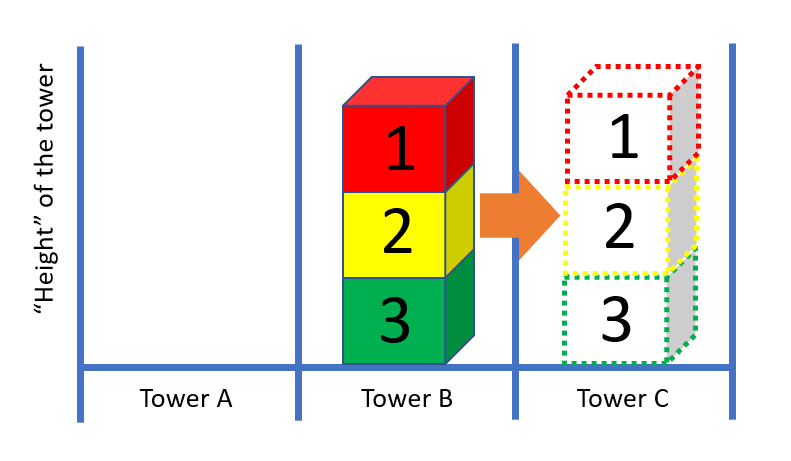
\includegraphics[scale=0.5]{image/lab3_3d_goal.png}
	\caption{\figlbl{towers} Standard Tower of Hanoi configuration with blocks stacked on top of each other.}
\end{figure}

\begin{figure}
	\centering
		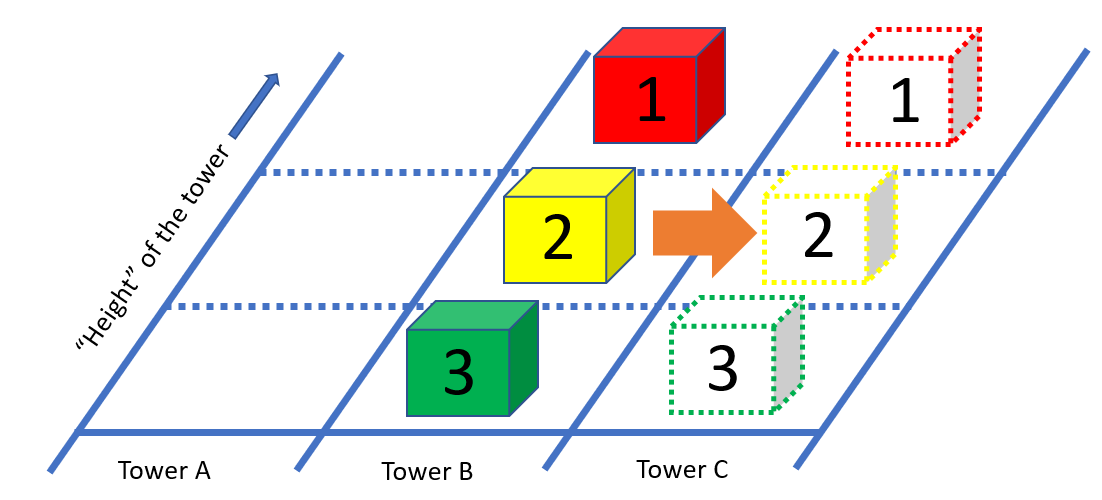
\includegraphics[scale=0.4]{image/lab3_2d_goal.png}
	\caption{\figlbl{towers2d} Example start and finish tower locations in the simulated version of the puzzle.}
\end{figure}

\begin{figure}
	\centering
		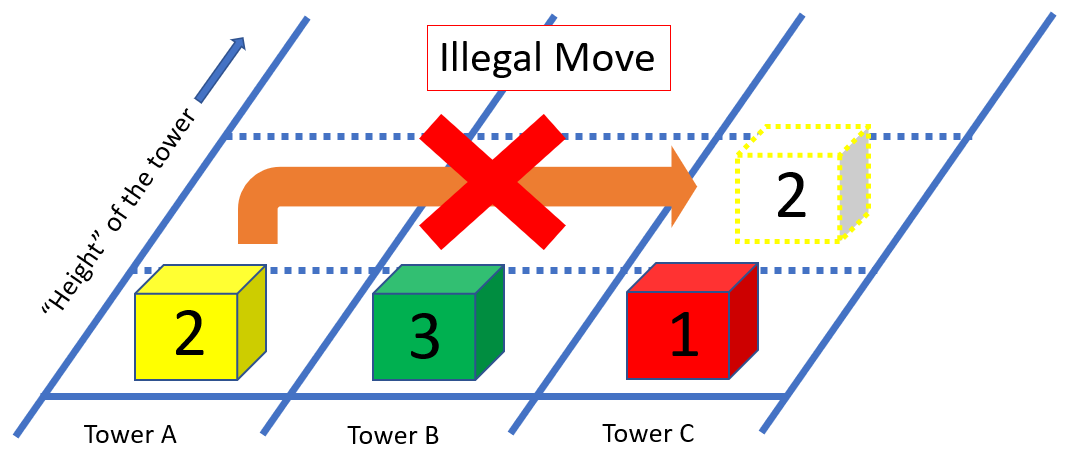
\includegraphics[scale=0.4]{image/lab3_2d_illegal.png}
	\caption{\figlbl{illegal} Example of an illegal move.}
\end{figure}

\begin{figure}
	\centering
		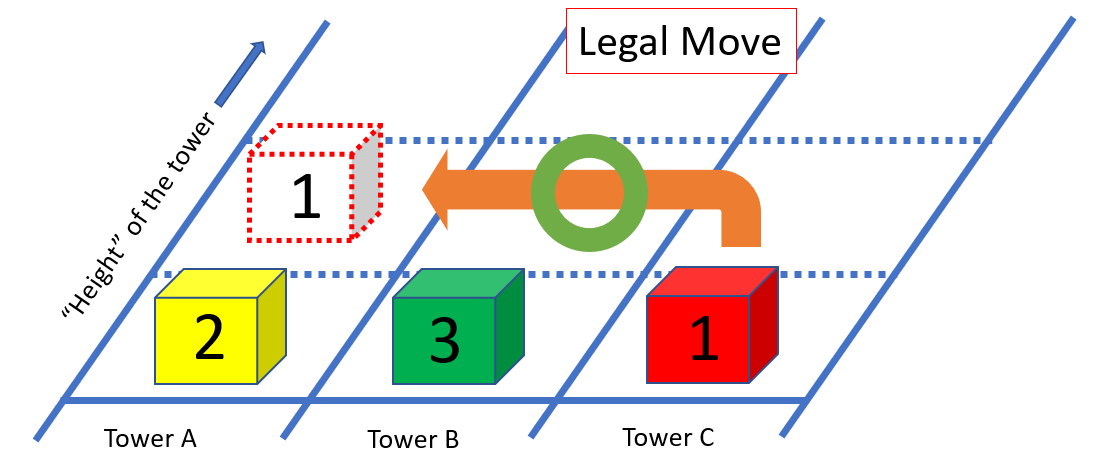
\includegraphics[scale=.4]{image/lab3_2d_legal.png}
	\caption{\figlbl{legal} Example of a legal move.}
\end{figure}



\newpage
\section{Procedure}
\begin{enumerate}
\item Create your own workspace as shown in Appendix \ref{cprog}.
\item Copy package \textbf{lab3pkg\_hanoi} into your workspace from \textbf{ECE470\_LAB}. All your coding work will be done in the script \textbf{lab3\_exec.py} with comments. Refer to \textbf{README.md} on how to run your code and robot!

\begin{itemize}
\item \textbf{lab3\_exec.py} a file in scripts folder with skeleton code to get you started on this lab. See Appendix \ref{cprog} for how to use basic ROS. Students are encouraged to make their own "cheat sheet" for some commonly used ROS and Linux commands. Also\
read carefully through the below section that takes you line by line through the starter code.  
\item \textbf{CMakeLists.txt} a file that sets up the necessary libraries and environment for compiling lab3\_exec.py.
\item \textbf{package.xml} This file defines properties about the package including package dependencies.
\item \textbf{README} To run lab3 code on real robot, please read it \textbf{FIRST}!
\item Every time you open a new terminal, make sure to source your workspace by running \textbf{source devel/setup.bash} in your workspace folder.
\end{itemize}

\item Modify \textbf{lab3\_exec.py} to prompt the user for the start and destination tower locations (you may assume that the user will not\
choose the same location twice) and move the blocks accordingly using the suction cup to grip the blocks.  The starter file performs basic motions 
but provides a function definition for moving blocks (\textbf{move\_block}). Once you understand
the starter code moving from one position to the next, clean up the code by completing the shell function \textbf{move\_block}.  
\textbf{move\_block} picks up a block from a tower and places it on another tower. You may also create other functions for prompting user input and solving the Tower of Hanoi problem given starting and ending locations but these are not required.  
\item Add one more feature to your program.  As you saw in Lab 1.5, the Coval device that is creating the vacuum for the gripper also senses
the level of suction being produced indicating if an item is in the gripper.  Recall that \textbf{Digital Input 0} are connected to
this feedback.  Use \textbf{Digital Input 0} to determine if a block is held by the gripper.  If no block is found where a block should be,
have your program exit, turn off the gripper, return home and print an error to the console.\\
To figure out how to do this with ROS you are going to have to do a bit of ``ROS" investigation.  Use ``\textbf{rostopic list}", ``\textbf{rostopic info}" and ``\textbf{rosmsg list}" to discover
what topic to subscribe and what message will be recieved in your subscribe callback function.  Once you find the topic and message run ``\textbf{rosmsg info}"
to figure out what variable you will need to read from the message sent to your callback function.  Just like the global variables thetas that
save the positions of the robot joints inside the call back \textbf{position\_callback()}, create global variables
to communicate to your code the state of \textbf{Digital Input 0}.  Normally once you figure out which message you will be using 
you need to import it in the \textbf{lab3\_header} file that defines this message.  The \textbf{lab3\_header} file has already imported it in \textbf{lab3\_header.py} for you.  Use the explanation below
and the given code in \textbf{lab3\_exec.py} that creates the subscription to \textbf{/joint\_states} and its callback function as a guide to subscribe to the rostopic
that publishes the IO status.     

\end{enumerate}

\section{Lab3\_exec.py Explained}
First open up \textbf{lab3\_exec.py} and read through the code and its comments as this is the latest version of Lab 2's starter code. Below is the same \textbf{lab3\_exec.py}\
file listing with code comments removed and possible small differences due to changes in the lab.  If you find a difference go with the actual \textbf{lab3\_exec.py}\
file as the correct version.  \textbf{lab3\_exec.py} is broken down into sections and described in more detail below.  

{\footnotesize
%\tiny{
%\begin{verbatim}[obeytabs,tabsize=4]
%\footnotesize{
\begin{verbatim}
import copy
import time
import rospy
import numpy as np
from lab3_header import *

# 20Hz
SPIN_RATE = 20 
    
# UR3 home location
home = np.radians([-87.42, -103.45, -72.77, -79.02, 89.95, 129.93])
    
# UR3 current position, using home position for initialization
current_position = copy.deepcopy(home)
    
thetas = [0.0, 0.0, 0.0, 0.0, 0.0, 0.0]
    
digital_in_0 = 0
analog_in_0 = 0
    
suction_on = True
suction_off = False
    
current_io_0 = False
current_position_set = False

Q = None
\end{verbatim}}

You can find \textbf{lab3\_header.py} in the \textbf{lab3pkg\_py/scripts} directory.  It includes all needed files to allow \textbf{lab3\_exec.py} to call ROS functionality.
\textbf{SPIN\_RATE} will be used as the publish rate to send commands to the ROS driver. This block also initializes positions such as the home position and a global variable to store the current position. There are also some other global variables for storing the input/feedback states and also some constants. You should use these global variables and constants in different functions to help you finish the task.

Q is a list that stores all the necessary waypoints for the robot to pick and place the blocks in order to solve the Tower of Hanoi. In each entry of Q[tower index][block height][above block/on block], there are six angles in radians that correspond to the arm's six joint angles. Q is defined as illustrated below:

\begin{figure}[h]
    \centering
    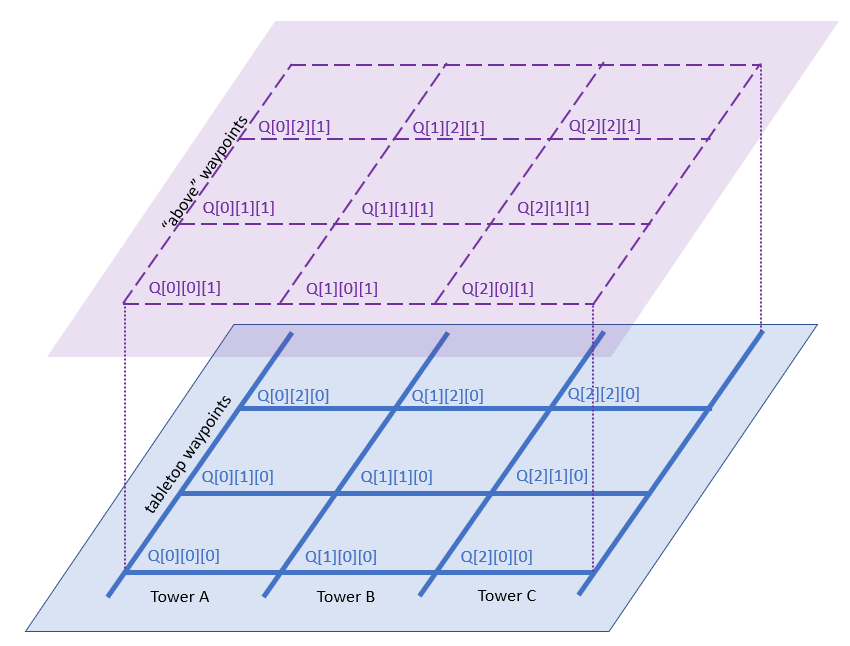
\includegraphics[scale=0.5]{image/lab3_waypoints.png}
    \caption{Waypoints Matrix Q}
\end{figure}
 
{\footnotesize
\begin{verbatim}
def position_callback(msg):

    global thetas
    global current_position
    global current_position_set

    thetas[0] = msg.position[0]
    thetas[1] = msg.position[1]
    thetas[2] = msg.position[2]
    thetas[3] = msg.position[3]
    thetas[4] = msg.position[4]
    thetas[5] = msg.position[5]

    current_position[0] = thetas[0]
    current_position[1] = thetas[1]
    current_position[2] = thetas[2]
    current_position[3] = thetas[3]
    current_position[4] = thetas[4]
    current_position[5] = thetas[5]

    current_position_set = True
\end{verbatim}}

This is \textbf{lab3\_node}'s callback function that is called when the \textbf{ur\_hardware\_interface} publishes new position data.  \textbf{ur\_hardware\_interface} publishes new
angle position data every 8ms, so this function \textbf{position\_callback} is run every 8ms.  
   
Next in \textbf{lab3\_exec.py} are the function \textbf{gripper()} and \textbf{move\_arm()}.  These functions are passed variables that are initialized at the beginning of the file. The program runs from the main function, so it will
be explained first and then we will come back to \textbf{gripper()} and \textbf{move\_arm()}.
   
{\footnotesize
\begin{verbatim}
def main():
    global home
    global Q
    global SPIN_RATE

    # Initialize ROS node
    rospy.init_node('lab3_node')

    # Initialize publisher for ur3e_driver_ece470/setjoint with buffer size of 10
    pub_setjoint = rospy.Publisher('ur3e_driver_ece470/setjoint',JointTrajectory,queue_size=10)
    
    # Initialize subscriber to /joint_states and callback fuction
    sub_position = rospy.Subscriber('/joint_states', JointState, position_callback)
\end{verbatim}}

To start as a ROS node the \textbf{rospy.init\_node()} function needs to be called.  Then the node needs to setup which other nodes it receives data from and which nodes\
it sends data to.  This code first specifies that it will be publishing a message to the ``\textbf{ur3e\_driver\_ece470}" node ``\textbf{setjoint}" subscriber.\
The message it will be sending is the \textbf{command} message which consists of\
the desired robot joint angles, the velocity of each joint and the acceleration of each joints.  Next \textbf{lab3\_node} subscribes to\
``\textbf{ur\_hardware\_interface}" node ``\textbf{joint\_states}" publisher.  Whenever new joint angles are\
ready to be sent, the callback function ``\textbf{position\_callback}" is called and passed the message \textbf{position} which\
contains the six joint angles.
As an exercise in lab, see if you can list the ``\textbf{ur3e\_driver\_ece470}", ``\textbf{ur\_hardware\_interface}" node and\
``\textbf{ur3e\_driver\_ece470/setjoint}" subscriber and ``\textbf{joint\_states}" publisher using the ``\textbf{rostopic list}" command in your \textbf{catkin\_ work directory}.  Also use ``\textbf{rostopic info}" to double\
check that ``\textbf{ur3e\_driver\_ece470/setjoint}" is a subscriber and ``\textbf{joint\_states}" is a publisher.  Also run ``\textbf{rosmsg list}" to find the messages.  

{\footnotesize
\begin{verbatim}   
    input_done = 0
    loop_count = 0
    
    while(not input_done):
        input_string = raw_input("Enter number of loops <Either 1 2 3 or 0 to quit> ")
        print("You entered " + input_string + "\n")
    
        if(int(input_string) == 1):
            input_done = 1
            loop_count = 1
        elif (int(input_string) == 2):
            input_done = 1
            loop_count = 2
        elif (int(input_string) == 3):
            input_done = 1
            loop_count = 3
        elif (int(input_string) == 0):
            print("Quitting... ")
            sys.exit()
        else:
            print("Please just enter the character 1 2 3 or 0 to quit \n\n")
	
\end{verbatim}}

This standard python code printing messages to the command prompt and receiving text input from the command prompt.  It loops until the correct data is input. 

{\footnotesize
\begin{verbatim}
    # Check if ROS is ready for operation
    while(rospy.is_shutdown()):
        print("ROS is shutdown!")

    rospy.loginfo("Sending Goals ...")
	
    loop_rate = rospy.Rate(SPIN_RATE)
\end{verbatim}}

Here the code waits for \textbf{roscore} to be executed and ready.  \textbf{rospy.loginfo} prints a message to the command prompt.  \textbf{rospy.Rate(SPIN\_RATE)} sets up a\
class \textbf{loop\_rate} that can be used to sleep the calling process.  The amount of time that the process will sleep is determined by the \textbf{SPIN\_RATE} parameter.\
In our case this is set to 20Hz or 50ms.  \textbf{loop\_rate} does not wake up 50 ms after it has been called, instead it wakes up the process every 50ms.  \textbf{loop\_rate}\
keeps track of the last time it was called to determine how long to sleep the process to keep a consistent rate.    
   
{\footnotesize
\begin{verbatim}
    move_block(pub_setjoint, pub_setio, start, 0, des, 2)

\end{verbatim}}

This moves the arm to a number of positions to give you a start at how to program the robot to move to different positions.  See the move\_arm
and gripper function definitions below.

{\footnotesize
\begin{verbatim}

    def move_arm(pub_setjoint, dest):
    msg = JointTrajectory()
    msg.joint_names = ["shoulder_pan_joint", "shoulder_lift_joint", 
       "elbow_joint","wrist_1_joint", "wrist_2_joint", "wrist_3_joint"]
    point = JointTrajectoryPoint()
    point.positions = dest
    point.time_from_start = rospy.Duration(2)
    msg.points.append(point)
    pub_setjoint.publish(msg)
    time.sleep(2.5)    

\end{verbatim}}

The \textbf{move\_arm()} function takes as parameters \textbf{pub\_setjoint}, which is the publisher to \textbf{ur3e\_driver\_ece470} commanding a new position for the robot to move
to. \textbf{dest} is the six joint angle destinations, in radians, that the robot will be commanded to move to.  
The code creates a variable \textbf{msg} which is the command message to be sent \textbf{ur3e\_driver\_ece470}.  \textbf{msg} is assigned the \textbf{joint\_names}, \textbf{positions} and \textbf{time\_from\_start}.
Next the \textbf{msg} is published to \textbf{ur3e\_driver\_ece470} with the \textbf{pub\_setjoint.publish(msg)} instruction.
\textbf{time.sleep(2.5)} will sleep 2.5s waiting for the robot getting to the commanded position.


% {\footnotesize
% \begin{verbatim}
% def gripper(pub_cmd, loop_rate, io_0):

%     global SPIN_RATE
%     global thetas
%     global current_io_0
%     global current_position

%     error = 0
%     spin_count = 0
%     at_goal = 0

%     current_io_0 = io_0

%     driver_msg = command()
%     driver_msg.destination = current_position
%     driver_msg.v = 1.0
%     driver_msg.a = 1.0
%     driver_msg.io_0 = io_0   
%     pub_cmd.publish(driver_msg)

%     while(at_goal == 0):

%         if( abs(thetas[0]-driver_msg.destination[0]) < 0.0005 and \
%             abs(thetas[1]-driver_msg.destination[1]) < 0.0005 and \
%             abs(thetas[2]-driver_msg.destination[2]) < 0.0005 and \
%             abs(thetas[3]-driver_msg.destination[3]) < 0.0005 and \
%             abs(thetas[4]-driver_msg.destination[4]) < 0.0005 and \
%             abs(thetas[5]-driver_msg.destination[5]) < 0.0005 ):

%             at_goal = 1
		
%         loop_rate.sleep()

%         if(spin_count >  SPIN_RATE*5):
%             pub_cmd.publish(driver_msg)
%             rospy.loginfo("Just published again driver_msg")
%             spin_count = 0

%         spin_count = spin_count + 1

%     return error
% \end{verbatim}}

% The \textbf{gripper()} function is very similar to the \textbf{move\_arm()} function above.  The same \textbf{pub\_cmd} and \textbf{loop-rate} are passed to \textbf{gripper()} but only the On/Off
% desired state of the suction cup gripper is the remaining parameter.  Looking at the \textbf{move\_arm()} function \textbf{gripper()} looks very similar but the
% robot joint destination is the current state of the arm so the robot is already at that position so it does not move.  All that the command
% changes is whether the suction gripper is On or Off by setting \textbf{driver\_msg.io\_0} equal to the passed parameter \textbf{bool io\_0}.  See the \textbf{move\_arm()}
% description for more details on this code.    


{\footnotesize
\begin{verbatim}
def move_block(pub_setjoint, pub_setio, start_loc, start_height, end_loc, end_height):
    global Q
\end{verbatim}}

The \textbf{move\_block()} function definition is provided and should be used to complete the assignment. Functions are useful when the same procedure is used many
times.  To move a block, multiple arm movements are necessary along with gripper
actuation. Instead of cluttering the main with many calls to \textbf{move\_arm} and \textbf{gripper()}, you will compartmentalize the calls in the \textbf{move\_block} function.
Use this function to compartmentalize moving a block from one tower to another. 
The start and end locations are integers given to tower positions and the heights are integers for blocks in the stack.


% \todo[inline]{A lot of this might change}

\section{Report}
Each student will submit a lab report using the guidelines given in the “ECE 470: How to Write a Lab Report” document.  Please be aware of the following:
\begin{itemize}
    \item Lab reports will be submitted online at \href{https://learn.intl.zju.edu.cn/webapps/login/}{BlackBoard}.
    \item The report will be due \textbf{Two} weeks after your lab session for Lab 2.  Exact times and dates can be seen on \href{https://learn.intl.zju.edu.cn/webapps/login/}{BlackBoard}.

\end{itemize}
Your report should include the following:
\begin{itemize}	
	\item Briefly explain the objective of the lab i.e. the goal and rules of Tower of Hanoi.  Images would greatly aid in this explanation.
	\item What was the focus of this lab? (Hint: ROS and implementing feedback)
	\item With that in mind you should cover the following (in detail):
	\begin{itemize}
		\item What is ROS and how does it work? (What kind of figure would help explain this?)
		\item How did you use the ROS commands (i.e. \textbf{rostopic list}, \textbf{rostopic info}, etc.) to complete your task?
		\item How did you implement feedback?
	\end{itemize}
	\item Make use of code snippets as needed to aid in your explanation
	\item \textbf{Read “ECE 470: How to Write a Lab Report” carefully so you know all the requirements.}
	\item Unless your TA gives other guidance, include your \textbf{lab3\_exec.py} code as an Appendix to your report	as described in lab report guidelines.
\end{itemize}

% \todo[inline]{Does this make sense schedule wise?  1 week after lab, they will be in their off week.  Are in-person demos optional?  I am not sure that I like just 1 week for demo, that is stricter than normal lab.}
\section{Demo}
% Demonstrations of your working code will either be done in-person or over Zoom.  They will be done live (i.e. no recordings) with your lab section TA.  Demos are due \textbf{2} weeks after your lab session.

% The default method of demonstrating your work will be via the simulation.  While we want to encourage in-person students to run their code on the real robot, due to time limitations, this may be difficult to do with your TA by the due date.  You can always run it for your own satisfaction at another time.
% \subsection{Demo Process}
Your TA will require you to run your program (at least) twice; on each run, the TA will specify a different set of start and destination locations for the tower.  They will also test that suction feedback has been implemented correctly.


\section{Grading}
\begin{itemize}
\item 80 points, successful demonstration.
\item 20 points, report.
\end{itemize}
